\documentclass{article}
\title{投資の数学 — 期待値から資金管理まで}
\author{TeX 図書館}

\begin{document}

\section{この教科書のために — 期待値思考とは}

「次の 1 回」の結果は運で決まります。しかし回数を重ねると、結果は\textbf{期待値と資金管理}にほぼ完全に支配されます。この教科書では、ギャンブルと投資に共通する数理を、例題を手で計算しながら学びます。

方針は 3 つです。

\begin{enumerate}
\item \textbf{すべては期待値に還元する}: 「なんとなく勝てそう」を数値に変換する練習をします。
\item \textbf{分散を敵として測る}: 期待値が同じでも、ばらつきが大きいほど破綻し近いことを数値で確かめます。
\item \textbf{賭け方も最適化対象}: 何% 賭けるかは、勝率と同じくらい重要な変数です(ケリー基準)。
\end{enumerate}

統計学入門や大学数学入門(本図書館の他の教科書)の内容を援用しますが、この 1 冊だけで完結するよう必要な部分は復習しながら進めます。

\begin{quote}
\textbf{【心構え】}\ この教科書は数学を学ぶためのものであり、特定の金融商品や手法を推奨するものではありません。実際の投資では手数料・税金・流動性など、ここで扱わない要因が期待値を大きく侵食します。
\end{quote}

\section{確率の復習 — 勝ち負けを数える}

\subsection{確率とオッズ}

事象 \(A\) の確率を \(p = P(A)\)、\(q = 1 - p\) とします。確率 \(p\) は「失敗に対する成功の比率」として\textbf{オッズ} \(p : q\) とも表せます。たとえば \(p = 0.25\) のオッズは \(1:3\) です。

ギャンブルの世界で「オッズ 3 倍」といった場合、通常は\textbf{配当の倍率}(払戻倍率)を指します。数学では区別が重要なので、本書では
\begin{itemize}
\item \(p\): 勝率
\item \(b\): \textbf{ペイアウト比}(勝ったときに賭け金の何倍を\textbf{利益}として得るか)
\end{itemize}
の 2 つを使って表現します。「オッズ 3 倍で勝てば元手 1 に対して 3 が戻る」設定は、利益が 2 の \(b = 2\) です。

\subsection{独立試行と連敗の確率}

独立な試行を繰り返すとき、\(n\) 連敗する確率は \(q^n\) です。

\begin{quote}
\textbf{【例】}\ 勝率 60\% のトレードで 5 連敗する確率は \(0.4^5 \approx 1.0\%\)。ほぼ起こらないように見えますが、年間 200 回のトレードで「どこかの 5 連続」を考えると、窓は 196 個あり \(196 \times 0.4^5 \approx 2\) 回程度は起こりうる計算になります。\textbf{「1 回も連敗しない」前提の運用設計は失敗します}。
\end{quote}

\begin{quote}
\textbf{【演習】}\ 勝率 40\% の戦略で 8 連敗する確率と、資金の 25\% を毎回賭けたとき 8 連敗後の資金の残率を計算せよ。
\end{quote}

\textbf{解答の指針:}\ 8 連敗の確率は \(0.6^8 \approx 1.7\%\)。残率は \(0.75^8 \approx 10\%\)。連敗は必ず来る前提で、破綻しない賭け幅を設計するのが第 6 節以降の主題です。

\section{期待値 — 長期の平均を支配する量}

\subsection{期待値の定義}

確率変数 \(X\) の期待値は \(E[X] = \sum_x x\, P(X = x)\) でした。賭けの文脈では「賭け金 1 単位あたりの期待損益」を主役にします。勝てば \(b\)、負ければ \(-1\) を得る賭けでは
\[ E = p \cdot b - q \cdot 1 = p(b + 1) - 1 \]
これを\textbf{期待値係数}と呼びます。\(E > 0\) なら長期的に有利、\(E = 0\) ならフェア、\(E < 0\) なら不利です。

\begin{quote}
\textbf{【例】}\ 勝率 25\%、当たれば 5 倍配当(\(b = 4\))の賭け。
\[ E = 0.25 \times 4 - 0.75 = 0.25 \]
1 賭けあたり賭け金の 25\% が期待値。毎回賭け金全体を賭けると、\(n\) 回後の期待資金は \(1.25^n\) 倍——ただしこれは\textbf{平均値}の話で、代表値ではありません(第 4 節の主題)。
\end{quote}

\subsection{イーブン系とハウスエッジ}

\(E = 0\) のゲーム(\textbf{イーブンゲーム})は、何回やっても期待損益がゼロ——しかし分散のせいで資金曲線は大きく暴れ、\textbf{破産}するプレイヤーが出ます。\(E < 0\) のゲームでは、続ける限り期待値の分だけ確実に削られます。

\begin{quote}
\textbf{【例:ルーレット】}\ ユーロルーレット(37 マス)で赤に 1 単位賭けると、\(p = 18/37\) で 1 単位の利益、\(q = 19/37\) で 1 単位の損失。
\[ E = \frac{18}{37} - \frac{19}{37} = -\frac{1}{37} \approx -0.027 \]
この約 2.7\% が\textbf{ハウスエッジ}。ゼロのマス 1 個が、プレイヤー全員の長期成績を静かにマイナスへ動かします。
\end{quote}

\begin{quote}
\textbf{【演習】}\ 勝率 45\%、\(b = 1.5\) のトレードの期待値係数を求め、ハウスエッジつきのゲームとの違いを述べよ。
\end{quote}

\textbf{解答の指針:}\ \(E = 0.45 \times 1.5 - 0.55 = 0.125\)。正の期待値。ルーレットと違い「やらないほうが良い」のではなく「分散を抑える賭け方(次々節)をすれば成長が望める」ゲームです。

\section{分散とリスク — ばらつきの代償}

\subsection{同じ期待値、異なる運命}

2 つの賭けを比較します。

\begin{center}
\begin{tabular}{|l|c|c|}
\hline
 & 賭け A(コイン配当) & 賭け B(10 倍配当) \\
\hline
勝率 \(p\) & 0.5 & 0.1 \\
ペイアウト比 \(b\) & 1 & 9 \\
期待値係数 \(E\) & 0 & 0 \\
\hline
\end{tabular}
\end{center}

どちらも \(E = 0\) のフェアゲームですが、分散は別物です。賭け A の分散は \(b^2 p + q - 0^2 = 1\)、賭け B は \((9^2)(0.1) + (0.9)(1) = 9\)。\textbf{9 倍}の差です。

分散が大きいと何が起きるか。大数の法則が期待値の方向に収束するまでに必要な試行回数が爆発的に増えます。理論的には「十分回数を重ねればトントン」でも、その回数に到達する前に\textbf{資金がゼロになる}(破産する)経路が大多数を占めます。

\subsection{ギャンブラーの破産}

\begin{quote}
\textbf{【定理:ギャンブラーの破産】}\ イーブンゲームですべての資金を賭け続けると、いつか必ず破産する(確率 1)。負の期待値ならなおさら、正の期待値でも賭け幅が大きすぎれば破産確率は無視できません。
\end{quote}

正の期待値(\(E > 0\))でも破産しうる、というのがこの節の最重要ポイントです。期待値が正でも「毎回全財産を賭ける」戦略は、1 回の負けでゲームから降ろされてしまい、長期の期待値を享受できません。\textbf{期待値は「賭けられる回数が十分ある」ときにのみ実現する}のです。

\begin{quote}
\textbf{【演習】}\ \(E = 0.25\)(前節の例)の賭けで、資金 100 単位の人が毎回 100 単位(全額)を賭けた。1 回目で破産する確率を求めよ。また毎回 10 単位を賭けた場合、9 連敗で資金が尽きる確率(\(q^9\))と比較せよ。
\end{quote}

\textbf{解答の指針:}\ 全額賭けは初手で \(q = 0.75\) の確率で終了。10 単位賭けなら \(0.75^9 \approx 7.5\%\) で尽きるが、その後の余力は残る設計次第。\textbf{賭け幅を小さくすることは、期待値を一切変えずに破産確率だけを下げる}操作です。

\section{オッズの読み方 — 市場価格から確率へ}

\subsection{逆関数としてのオッズ}

オッズ(配当倍率)は市場がつけた「確率の推定値」を逆算できます。公正オッズなら \(p_{\text{implied}} = 1 / O\)(\(O\) は配当倍率)。オッズ 4.0 の馬券は、市場評価で勝率 25\% ということです。

現実のオッズには\textbf{マージン}(控除率)が含まれます。ブックメーカーは全結果の公正オッズの合計を 1 未満に設定します。

\begin{quote}
\textbf{【例】}\ 2 頭立てのレースでオッズ(配当倍率)1.8 と 2.0 がついたとします。各結果の逆算確率は \(1/1.8 = 0.556\) と \(1/2.0 = 0.500\) で、合計は \(1.056\)。公正なら合計はちょうど 1 になるはずなので、\textbf{超過分 5.6\% がブックメーカーの控除}(マージン)です。マージンを差し引いて初めて「市場の推定勝率」が得られ、プレイヤー側の期待値はその分だけ押し下げられています。
\end{quote}

\subsection{バリューベット}

自分の推定勝率 \(\hat{p}\) が市場の逆算勝率より十分に高く、\(E = \hat{p}(b+1) - 1 > 0\) となるときだけ賭ける、という意思決定を\textbf{バリューベット}といいます。

\begin{quote}
\textbf{【演習】}\ オッズ 2.9 の試合を「勝率 40\%」と推定した。\(\hat{p} = 0.45\) と推定した場合とそれぞれ期待値係数を計算し、賭けるべきか判断せよ。
\end{quote}

\textbf{解答の指針:}\ \(b = 1.9\)。\(\hat{p} = 0.40\) では \(E = 0.40 \times 2.9 - 1 = 0.16 > 0\) で賭け候補。\(\hat{p} = 0.45\) なら \(E = 0.305\) でより有利。\textbf{期待値を動かすのは賭け方が市場の推定より正確であること}であり、推定の信頼性(サンプル数・モデル)が全ての土台です。

\section{ケリー基準 — 最適な賭け割合}

\subsection{成長率の最大化}

毎回資金の割合 \(f\) を賭けると、勝敗で資金は \(1 + bf\) 倍、\(1 - f\) 倍になります。\(n\) 回後の資金の対数の平均(長期成長率)は
\[ g(f) = p \ln(1 + bf) + q \ln(1 - f) \]
これを最大化する \(f^*\) が\textbf{ケリー基準}です。微分して \(g'(f) = 0\) とおくと
\[ f^* = \frac{bp - q}{b} = \frac{p(b+1) - 1}{b} = \frac{E}{b} \]
つまり\textbf{期待値係数をペイアウト比で割ったもの}が最適賭け割合です。

\begin{figure}[h]
\centering
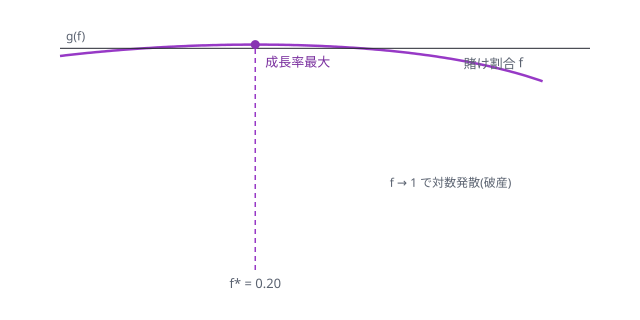
\includegraphics[width=0.8\textwidth]{figures/kelly.svg}
\caption{勝率 60\%、\(b = 1\) の賭けの成長率曲線。\(f^* = 0.2\) で最大となり、\(f \to 1\) で対数発散的に悪化する。}
\end{figure}

\begin{quote}
\textbf{【例】}\ 勝率 60\%、\(b = 1\)(オッズ 2 倍)の賭け。
\[ f^* = \frac{1 \times 0.6 - 0.4}{1} = 0.2 \]
資金の 20\% を賭けるのが長期成長率を最大化します。グラフから読める通り、\(f = 0.4\)(2 倍のオーバーベット)では成長率はほぼゼロに落ち、\(f = 0.6\) では\textbf{マイナス}です。\textbf{オーバーベットは期待値が正でも資金を減らす}。
\end{quote}

\subsection{半ケリーと推定誤差}

\(f^*\) の計算には「\(p\) と \(b\) が正確に分かっている」ことが前提ですが、実戦の \(p\) は推定値であり誤差を含みます。勝率を楽観しすぎた推定でフルケリーを賭け続けると、実態が悪い場合にオーバーベットになります。

そこで実務では \(\frac{1}{2} f^*\) や \(\frac{1}{4} f^*\)(\textbf{半ケリー}・\textbf{クォーターケリー})を使うのが定石です。成長率は最大値よりやや下がりますが、成長率曲線の頂点付近は平坦なので\textbf{損失は小さく、破産リスクは大幅に減る}という、極めて良いトレードオフになります。

\begin{quote}
\textbf{【演習】}\ \(b = 2\), \(p = 0.45\) の賭けの \(f^*\) を求め、半ケリーの金額を資金 100 万円で計算せよ。
\end{quote}

\textbf{解答の指針:}\ \(f^* = (2 \times 0.45 - 0.55)/2 = 0.175\)。半ケリーは 8.75\%、つまり 8 万 7500 円。

\section{資金管理と破産確率}

\subsection{固定比率と固定額}

代表的な資金管理を 2 つ挙げます。

\begin{itemize}
\item \textbf{固定額方式}: 常に同じ金額を賭ける。破産しにくいが、資金が増えても成長しない(線形成長)。
\item \textbf{固定比率方式}: 資金の一定割合を賭ける。資金に比例して成長(指数成長)し、負けても賭け幅が自動的に縮む。\textbf{ケリー的発想の実践形}です。
\end{itemize}

固定比率 \(f\) の賭けを \(n\) 回続けたとき、\(w\) 勝 \(n - w\) 負けの資金は \(F = (1 + bf)^w (1 - f)^{n - w}\) 倍です。順番に依存しない——\textbf{割合運用では勝ち負けの順序が最終資金を決めない}(この性質が破産耐性の源泉です)。

\subsection{破産確率の見積もり}

破産確率を厳密に計算するのは難しいので、設計上は次の 2 つの近似を使います。

\begin{enumerate}
\item \textbf{最悪連敗シナリオ}: 資金の \(f\) を賭ける場合、\(n\) 連敗で資金が \((1 - f)^n\) に落ちる。\((1 - f)^{n} < \varepsilon\)(耐えられる最低残率)となる \(n\) を数え、\(q^n\) と自分の運用回数から発生可能性を判断する。
\item \textbf{ドローダウン分布}: シミュレーション(次節)で最大下落幅の分布を直接見る。
\end{enumerate}

\begin{quote}
\textbf{【例】}\ \(f = 0.1\)、勝率 50\%、\(b = 1\) の場合、10 連敗(確率 \(0.5^{10} \approx 0.1\%\))で資金 \(0.9^{10} \approx 35\%\) 残存。1000 回運用すれば 10 連敗はほぼ確実に一度は起きるが、35\% のドローダウンで生き残れるなら設計は成立する。一方 \(f = 0.25\) では 10 連敗で \(0.75^{10} \approx 5.6\%\) まで落ちる。\textbf{同じ連敗で、生き残れるかどうかが賭け幅で決まる}。
\end{quote}

\begin{quote}
\textbf{【演習】}\ 「1 回のリスクは資金の 1〜2\% まで」という実務の規則を、\(f\) が小さいほど \((1-f)^n\) の劣化が緩やかになることから説明せよ。
\end{quote}

\textbf{解答の指針:}\ \(f = 0.02\) なら 50 連敗しても \(0.98^{50} \approx 36\%\) 残存し、回復の余地が十分ある。小さな \(f\) は「負けの連鎖を一時的な事件で済ませる」設計であり、正の期待値さえあれば回復は数学的に保証される。

\section{モンテカルロシミュレーション}

理論式では追いきれないのは、\textbf{経路依存}の問いです。破産・ドローダウン・「最大連敗は何回か」は、資金曲線の経路によって変わります。そこで乱数を大量に発生させて分布を直接観察する\textbf{モンテカルロ法}を使います。

\begin{lstlisting}[language=Python]
import random, statistics

def simulate(f=0.1, p=0.55, b=1.0, n=200, trials=10000):
    finals, maxdds = [], []
    for _ in range(trials):
        equity = 1.0
        peak = 1.0
        maxdd = 0.0
        for _ in range(n):
            if random.random() < p:
                equity *= 1 + b * f   # 勝ち
            else:
                equity *= 1 - f       # 負け
            peak = max(peak, equity)
            maxdd = max(maxdd, 1 - equity / peak)  # ドローダウン
        finals.append(equity)
        maxdds.append(maxdd)
    return finals, maxdds

finals, maxdds = simulate()
print("最終資金の中央値:", statistics.median(finals))
print("破産(80%損失)した経路の割合:",
      sum(1 for x in finals if x < 0.2) / len(finals))
print("最大ドローダウンの90%タイル:", statistics.quantiles(maxdds, n=10)[-1])
\end{lstlisting}

勝率 55\%、\(b = 1\)、\(f = 0.1\) の設定では、ケリー比 \(f^* = 0.1\) ちょうどです。シミュレーションを動かすと、\textbf{中央値は増えるのに平均は少数の幸運な経路に引っ張られる}こと、そして 200 回の中の最大ドローダウンが思ったより深いことが観察できます。解析解が難しい問いに対する、モンテカルロ法の典型例です。

\begin{quote}
\textbf{【演習】}\ 上のシミュレーションの \(f\) を \(0.2\)(2 倍オーバー)に変えて実行し、最終資金の中央値と破産率がどう変わるか確かめよ。
\end{quote}

\textbf{解答の指針:}\ 中央値は \(f = 0.1\) のときより明確に低くなり、破産率(80\% 損失)が 0 から大きく上昇する。期待値が正でも、賭け幅の倍増で長期成長は悪化する——ケリーの理論と一致する結果が経験的に確認できる。

\section{期待値の落とし穴 — 数理が教える認知バイアス}

最後に、数理の視点から見える意思決定の落とし穴を整理します。

\begin{enumerate}
\item \textbf{ギャンブラーの誤謬}: 独立試行で「次は負けているから勝つ番」。連の情報は次の試行の確率を変えません。変わるのは\textbf{資金}だけです。
\item \textbf{サンクコスト}: すでに失った資金を取り戻そうと賭け幅を上げるのは、期待値計算とは無関係の行動です。考えるべきは\textbf{現在の資金に対する}次の賭けの期待値です。
\item \textbf{マーティンゲール}: 負けるごとに賭け額を倍にして前の負けを取り返す戦略。負けが続くと賭け額が指数関数的に増え、\textbf{有限な資金では必ず破綻}します。期待値はそもそも負のままなので、途中の「勝率の高さ」は幻想です。
\item \textbf{小標本への過信}: 20 回の成績では期待値を推定できません(標準誤差が大きすぎる)。戦略の評価には十分な試行数と、第 9 節のモンテカルロ的な「運の範囲」の確認が必要です。
\item \textbf{ハウスエッジの軽視}: 期待値 −2.7\% のゲームは、1 回あたりの差が小さく見えても\textbf{回数に比例して確実に}蓄積します。ボリューム(賭け回数 × 賭け幅)は期待値損失の乗数です。
\end{enumerate}

\begin{quote}
\textbf{【演習】}\ マーティンゲール(初期賭け 1、負けるたびに 2 倍)で、9 連敗すると累積賭け額がいくらになるか計算し、資金 1000 の人がこの戦略を続けられるか述べよ。
\end{quote}

\textbf{解答の指針:}\ 累積賭け額は \(1 + 2 + 4 + \cdots + 2^8 = 511\)。9 連敗(確率は負け率に依存)した時点で 511 を失っており、次の賭けには 512 必要で資金 1000 ではほぼ破綻。勝率は高いが\textbf{1 回の破綻で全てを失う}構造です。

\section{おわりに — 期待値と仲良くなる}

この教科書の流れを振り返ります。

\textbf{期待値}(第 3 節)が長期の平均を決め、\textbf{分散}(第 4 節)がその平均に到達できるかどうかを左右し、\textbf{賭け幅}(第 6・7 節)が破産確率を制御する。そして \textbf{シミュレーション}(第 8 節)が理論と現実の橋渡しをします。共通する教訓はひとつです。

\begin{quote}
\textbf{「期待値が正であること」と「資金が増えること」は別の問題である。後者には資金管理が要る。}
\end{quote}

次の一歩としては、確率過程(マルコフ連鎖・ランダムウォーク)、統計学入門の仮説検定による戦略評価、そして実際のデータでのバックテストが自然な延長線です。この図書館の『統計学入門』『大学数学入門』と併読すると、数理の全体像がつながります。

\begin{quote}
\textbf{【総合演習】}
\begin{enumerate}
\item 勝率 55\%、\(b = 1\) の賭けの期待値係数とケリー比を求めよ。
\item 上の設定で毎回資金の 20\% を賭け、10 連敗したときの資金残率を求めよ。
\item 「オッズ 2.9 の試合を勝率 45\% と推定した」とき、賭けるべきか期待値で判断せよ。
\end{enumerate}
\end{quote}

\textbf{解答の指針:}\ 1. \(E = 0.55 - 0.45 = 0.1\)、\(f^* = E/b = 0.1\)。2. \(0.8^{10} \approx 10.7\%\)。3. \(E = 0.45 \times 2.9 - 1 = 0.305 > 0\) なので賭け候補(推定の信頼性に応じて半ケリー以下の賭け幅で)。

\end{document}
